\documentclass{article}
\usepackage[UKenglish]{babel}
\usepackage[UKenglish]{isodate}
\usepackage[utf8]{inputenc}
\usepackage{fullpage}

\usepackage{mathtools}
\usepackage{amsthm}
\usepackage{mathrsfs}
\usepackage{amsfonts}

\usepackage[linesnumbered,ruled,vlined]{algorithm2e}
\usepackage{tikz}
\usepackage[capitalize]{cleveref}

\usetikzlibrary{fit,positioning,trees,cd}
\usetikzlibrary{shapes}
\usetikzlibrary{arrows}
\usetikzlibrary{arrows.meta}

\crefname{algocf}{algorithm}{Algorithms}
\Crefname{algocf}{Algorithm}{Algorithms}

\newtheorem{theorem}{Theorem}
\theoremstyle{definition}
\newtheorem{definition}{Definition}
\newtheorem{example}{Example}
\newtheorem{observation}{Observation}
\theoremstyle{remark}
\newtheorem*{remark}{Remark}

\makeatletter
\newcommand\incircbin
    {%
      \mathpalette\@incircbin
    }
    \newcommand\@incircbin[2]
                          {%
                            \mathbin%
                                {%
                                  \ooalign{\hidewidth$#1#2$\hidewidth\crcr$#1\bigcirc$}%
                                }%
                          }
                          \newcommand{\oland}{\incircbin{\land}}
                          \newcommand{\olor}{\incircbin{\lor}}
                          \newcommand{\Contradiction}{\incircbin{\bot}}
                          \newcommand{\Tautology}{\incircbin{\top}}
                          \newcommand{\Smoothing}{\incircbin{}}
                          \newcommand{\Unit}{\incircbin{1}}
                          \makeatother

\newcommand\pfun{\mathrel{\ooalign{\hfil$\mapstochar\mkern5mu$\hfil\cr$\to$\cr}}}
\newcommand\mdoubleplus{\mathbin{+\mkern-10mu+}}

\DeclareMathOperator{\Compile}{\textsc{Compile}}
\DeclareMathOperator{\CR}{\textsc{CR}}
\DeclareMathOperator{\DR}{\textsc{DR}}
\DeclareMathOperator{\IE}{\textsc{IE}}
\DeclareMathOperator{\Reff}{\textsc{Ref}}
\DeclareMathOperator{\wwp}{w}
\DeclareMathOperator{\wwn}{\overline{w}}

\DeclareMathOperator{\dom}{dom}
\DeclareMathOperator{\Imm}{Im}
\DeclareMathOperator{\Doms}{Doms}
\DeclareMathOperator{\size}{\sigma}
\DeclareMathOperator{\Vars}{Vars}
\DeclareMathOperator{\WMC}{WMC}
\DeclareMathOperator{\gr}{gr}

\title{Recursive Solutions to First-Order Model Counting}

\begin{document}
\maketitle

\section{Definitions}

\begin{figure}[t]
  \centering
  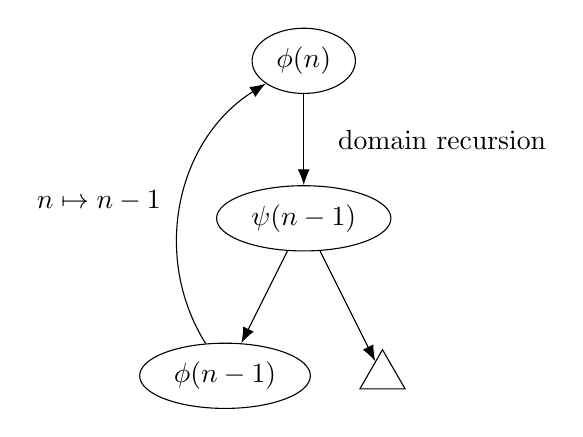
\begin{tikzpicture}[triangle/.style = {regular polygon, regular polygon sides=3}]
    \node[draw,ellipse] (a) at (0, 0) {$\phi(n)$};
    \node[draw,ellipse] (b) at (0, -2) {$\psi(n-1)$};
    \node[draw,ellipse] (c) at (-1, -4) {$\phi(n-1)$};
    \node[draw,triangle] (d) at (1, -4) {};
    \draw[-{Latex[length=2mm]}] (a) -- (b) node [midway,xshift=50] {domain recursion};
    \draw[-{Latex[length=2mm]}] (b) -- (c);
    \draw[-{Latex[length=2mm]}] (b) -- (d);
    \draw[-{Latex[length=2mm]}] (c) to [bend left=45] node [midway,xshift=-30] () {$n \mapsto n-1$} (a);
  \end{tikzpicture}
  \caption{An illustration of the main idea. TODO: refer to this in the introduction.}
\end{figure}

\paragraph{Things I might need to explain.}
\begin{itemize}
\item atom, (positive/negative) literal, constant, predicate, variable, literal variable, clause, unit clause
\item $\Vars$, $\Vars(c) = \Vars(L) \cup \Vars(C)$
\item $\Doms$ on both formulas and clauses. $\Doms(c) = \Imm \delta_c$, and $\Doms(\phi) = \bigcup_{c \in \phi} \Doms(c)$.
\item maybe: notation for partial function, notation for powerset, notation for disjoint union
\item $\WMC$, $\wwp$, $\wwn$, $\Imm$
\item two parts: compilation and inference.
\item introduce and use arrows for bijections, injections, set inclusions, etc.
\item $\emptyset$ for an empty partial map.
\item notation for variable substitution for literal and constraint sets: $S[x/V]$, where $S$ is the set, $V$ is a set of variable, and $x$ is the new constant or variable. Note that for constraint sets this could mean that a variable and a constant need to switch places.
\item During inference, there is a domain size map $\size\colon \mathcal{D} \to \mathbb{N}_0$.
\item $\sqcup$ for both sets and functions. TODO: I think I use $\cup$ elsewhere.
\item mention which rules are in $\Gamma$ and which ones are in $\Delta$ (and why tryCache has to be in $\Delta$).
\end{itemize}

\paragraph{TODO}
\begin{itemize}
\item should I always say `compilation rule' instead of `operator'?
\item maybe $\pi$ is global enough to have a more unique name
\item capitalise variable names.
\item maybe introduce/use notation for vertices, edges of a graph
\item maybe put each function into its own algorithm environment, using the caption for the function name
\end{itemize}

Most of the definitions here are adaptations/formalisations of \cite{DBLP:conf/ijcai/BroeckTMDR11} and the corresponding code.

\begin{definition}
  A \emph{domain} is a symbol for a finite set.\footnote{In the context of functions, the domain of a function $f$ retains its usual meaning and is denoted $\dom(f)$.} Let $\mathcal{D}$ be the set of all domains and $\mathcal{C} \subset \mathcal{D}$ be the subset of domains introduced as a consequence of constraint removal. Note that both sets (can) expand during the compilation phase.

Let $\pi\colon \mathcal{D} \pfun \mathcal{D}$ be a partial endomorphism on $\mathcal{D}$ that denotes the \emph{parent} relation, i.e., if $\pi(d) = e$ for some $d, e \in \mathcal{D}$, then we call $e$ the parent (domain) of $d$, and $e$ a child of $d$. Intuitively, $\pi$ arranges all domains into a forest---thus, we often use graph theoretical terminology to describe properties of and relationships between domains.
\end{definition}

\begin{definition}
An \emph{(inequality) constraint} is a pair $(a, b)$, where $a$ is a variable, and $b$ is either a variable or a constant.
\end{definition}

\begin{definition}
  A \emph{clause} is a triple $c = (L, C, \delta_c)$, where $L$ is the set of literals, $C$ is a set of inequality constraints, and $\delta_c\colon \Vars(c) \to \mathcal{D}$ is a function that maps all variables in $c$ to their domains such that if $(x, y) \in C$ for some variables $x$ and $y$, then $\delta_c(x) = \delta_c(y)$. Equality of clauses is defined in the usual way (i.e., all variables, domains, etc. must match). TODO: we will always use this subscript notation for the $\delta$'s. 
\end{definition}

A \emph{formula} is a set of clauses.

We use hash codes to efficiently check whether a recursive relationship between two formulas is plausible. (It is plausible if the formulas are equal up to variables and domains.) The hash code of a clause $c = (L, C, \delta_c)$ combines the hash codes of the sets of constants and predicates in $c$, the numbers of positive and negative literals, the number of inequality constraints $|C|$, and the number of variables $|\Vars(c)|$. The hash code of a formula $\phi$ combines the hash codes of all its clauses and is denoted $\#\phi$.

\begin{definition}
  Let $\gr(\cdot; \sigma)$ be the function (parameterised by the domain size function $\size$) that takes a clause $c = (L, C, \delta)$ and returns the number of ways the variables in $c$ can be replaced by elements of their respective domains in a way that satisfies the inequality constraints.\footnote{Note that the literals of the clause have no effect on $\gr$.} Formally, for each variable $v \in \Vars(c)$, let $C_v = \{ w \mid (u, w) \in C \setminus \Vars(c)^2 \text{, }u \ne v \}$ be the set of (explicitly named) constants that $v$ is permitted to be equal to. Then
  \[
  \gr(c; \sigma) \coloneqq \left|\left\{\, (e_v)_{v \in \Vars(c)} \in \prod_{v \in \Vars(c)} C_v \sqcup [\sigma(\delta(v)) - |C_v|] \;\middle|\; \right.\right. e_u \ne e_w \text{ for all } (u, w) \in C \cap \Vars(c)^2 \left.\left. \vphantom{\prod_{v \in \Vars(c)}} \,\right\}\right|
  \]
  for any clause $c$. (Here, $[n] \coloneqq \{\,1, 2, \dots, n\,\}$ for any non-negative integer $n$.)
\end{definition}

TODO: I'm already using the square brackets to denote lists.

TODO: how does the algorithm prevent the number in $[\cdot]$ from being negative?

\section{Search/Compilation}

\begin{definition}
  A \emph{first-order deterministic decomposable negation normal form computational graph} (FCG) is a (weakly connected) directed graph with a a single source, node labels, and ordered direct successors. We denote an FCG as $G = (V, s, N^+, \lambda)$, where $V$ is the set of nodes, $s \in V$ is the source, $N^+$ is the direct successor function that maps each node in $V$ to a list that contains either other nodes in $V$ or $\star$, which means that the target of the edge is yet to be determined, and $\lambda\colon V \to \mathcal{L}$ is the vertex-labelling function with some codomain $\mathcal{L}$, which is assumed to be the same for all FCGs. For each $v \in V$, the length of the list $N^+(v)$ is determined by $\lambda(v)$.

\end{definition}

\paragraph{TODO.}
\begin{itemize}
\item explain the connection to the algebraic formalism (or just don't use it). % We will also use algebraic notation to describe (parts of) circuits: circuittype_parameters(nodes pointed to by the outedges)
\item define `an FCG for a formula'
\item vertex or node, $v$ or $n$?
\item what notation for lists (a.k.a. sequences) am I going to use? $\mdoubleplus$ for concatenation (of both two lists and an element to a list), $\in$ for (in-order) enumeration, $[]$ for an empty list, $[x]$ for a list with one element, $|L|$ for the length of the list, and $h : t$ to denote a list with first element (a.k.a. head) $h$ and remaining list (a.k.a. tail) $t$. Also add an example of the list comprehension notation.
\end{itemize}

\begin{definition}
  A \emph{state} (of the search for an FCG for a given formula) is a tuple $(G, C, L)$, where:
  \begin{itemize}
  \item $G$ is an FCG (can be \texttt{null}),
  \item $C$ is a compilation cache that maps integers to sets of pairs $(\phi, n)$, where $\phi$ is a formula, and $n$ is a node of $G$ (which is used to identify opportunities for recursion),
  \item and $L$ is a list of formulas (that are yet to be compiled). (Note that the order is crucial!)
  \end{itemize}
\end{definition}

\begin{definition}
  A (compilation) \emph{rule} is a function that takes a formula and returns a set of $(G, L)$ pairs, where $G$ is a (potentially \texttt{null}) FCG, and $L$ is a list of formulas. TODO: add an example showing that it's usually an FCG with one node and a bunch of $\star$'s marking a fixed number of outedges.
\end{definition}

We assume that if there is a pair $(\texttt{null}, L)$ in the set returned by a rule, then $|L| = 1$, i.e., the rule transformed the formula without creating any nodes.

\begin{algorithm}[t]
  \caption{The (main part of the) search algorithm}
  \label{alg:search}
  \SetKwProg{Fn}{Function}{:}{}
  \SetKwData{solutions}{solutions}
  \SetKwFunction{applyGreedyRules}{applyGreedyRules}
  \SetKwFunction{applyAllRules}{applyAllRules}
  \SetKwFunction{put}{put}
  \SetKwFunction{get}{get}
  \SetKwFunction{emptyy}{empty}
  \KwIn{a formula $\phi_0$}
  \KwResult{all found FCGs for $\phi_0$ are in the set \solutions}
  $\solutions \gets \emptyset$\;
  $C_0 \gets \emptyset$\;
  $(G_0, C_0, L_0) \gets \applyGreedyRules{$\phi_0$, $C_0$}$\;
  \lIf{$L_0 = []$}{$\solutions \gets \{\, G_0 \,\}$}
  \Else{
    $q \gets \text{an empty queue of states}$\;
    $q.\put{$(G_0, C_0, L_0)$}$\;
    \While{{\bf not} $q.\emptyy{}$}{
      \ForEach{state $(G, C, L) \in \applyAllRules{$q.\get{}$}$}{
        \lIf{$L = []$}{$\solutions \gets \solutions \cup \{\, G \,\}$}
        \lElse{$q.\put{$(G, C, L)$}$}
      }
    }
  }
\end{algorithm}

\begin{algorithm}
  \caption{Functions used in \cref{alg:search} for applying compilation rules}
  \label{alg:apply}
  \SetKwProg{Fn}{Function}{:}{}
  \SetKwData{newStates}{newStates}
  \SetKwFunction{applyGreedyRules}{applyGreedyRules}
  \SetKwFunction{applyAllRules}{applyAllRules}
  \SetKwFunction{applyGreedyRulesToAllFormulas}{applyGreedyRulesToAllFormulas}
  \SetKwFunction{mergeFcgs}{mergeFcgs}
  \SetKwFunction{updateCache}{updateCache}
  \KwData{a set of greedy rules $\Gamma$}
  \KwData{a set of non-greedy rules $\Delta$}
  \Fn{\applyGreedyRules{$\phi$, $C$}}{
    \ForEach{rule $r \in \Gamma$}{
      $S \gets r(\phi)$\;
      \If{$S \ne \emptyset$}{
        $(G, L) \gets \text{any element of } S$\;
        \lIf{$G = {\normalfont \texttt{null}}$}{\Return{\applyGreedyRules{the only element of $L$, $C$}}}
        \Else{
          $(V, s, N^+, \lambda) \gets G$\;
          $C \gets \updateCache(C, \phi, s)$\;
          \Return{\applyGreedyRulesToAllFormulas{$G$, $C$, $L$}}\;
        }
      }
    }
    \Return{$({\normalfont \texttt{null}}, C, [\phi])$}\;
  }
  \Fn{\applyGreedyRulesToAllFormulas{$G$, $C$, $L$}}{
    $(V, s, N^+, \lambda) \gets G$\;
    $N^+(s) \gets []$\;
    $L' \gets []$\;
    \ForEach{formula $\phi \in L$}{
      $(G', C, L'') \gets \applyGreedyRules{$\phi$, $C$}$\;
      $L' \gets L' \mdoubleplus L''$\;
      \lIf{$G' = {\normalfont \texttt{null}}$}{$N^+(s) \gets N^+(s) \mdoubleplus [\star]$}
      \Else{
        $(V', s', N', \lambda') \gets G'$\;
        $V \gets V \sqcup V'$\;
        $N^+ \gets N^+ \sqcup N'$\;
        $N^+(s) \gets N^+(s) \mdoubleplus [s']$\;
        $\lambda \gets \lambda \sqcup \lambda'$\;
      }
    }
    \Return{$((V, s, N^+, \lambda), C, L')$}\;
  }
  \Fn{\applyAllRules{$s$}}{
    $(G, C, L) \gets s$\;
    $\phi : T \gets L$\;
    $(G', C', L') \gets \text{a copy of } s$\;
    $\newStates \gets []$\;
    \ForEach{rule $r \in \Delta$}{
      \ForEach{$(G'', L'') \in r(\phi)$}{
        \lIf{$G'' = {\normalfont \texttt{null}}$}{$\newStates \gets \newStates \mdoubleplus \applyAllRules{$(G', C', L'')$}$}
        \Else{
          $(V, s, N^+, \lambda) \gets G''$\;
          $C' \gets \updateCache{$C'$, $\phi$, $s$}$\;
          $(G'', C', L'') \gets \applyGreedyRulesToAllFormulas{$G''$, $C'$, $L''$}$\;
          \lIf{$G' = {\normalfont \texttt{null}}$}{$\newStates \gets \newStates \mdoubleplus [(G'', C', L'' \mdoubleplus T)]$}
          \lElse{$\newStates \gets \newStates \mdoubleplus [(\mergeFcgs{$G'$, $G''$}, C', L'' \mdoubleplus T)]$}
        }
      }
      $(G', C', L') \gets \text{a copy of } s$\;
    }
    \Return{\newStates}\;
  }
\end{algorithm}

\begin{algorithm}
  \caption{Helper functions used by \cref{alg:apply}}
  \label{alg:helpers}
  \SetKwProg{Fn}{Function}{:}{}
  \SetKwFunction{mergeFcgs}{mergeFcgs}
  \SetKwFunction{updateCache}{updateCache}
  \Fn{\updateCache{$C$, $\phi$, $v$}}{
    \lIf{$\#\phi \not\in \dom(C)$}{\Return{$C \cup \{\, \#\phi \mapsto (\phi, v) \,\}$}}
    \lIf{there is no $(\phi', v') \in C(\#\phi)$ such that $v' = v$}{$C(\#\phi) \gets (\phi, v) \mdoubleplus C(\#\phi)$}
    \Return{$C$}\;
  }
  \Fn{\mergeFcgs{$G = (V, s, N^+, \lambda)$, $G' = (V', s', N', \lambda')$, $r = s$}}{
    \lIf{$\lambda(r) = \textsc{Ref}$}{\Return{\normalfont \texttt{null}}}
    \ForEach{$t \in N^+(r)$}{
      \If{$t = \star$}{
        replace $t$ with $s'$ in $N^+(r)$\;
        \Return{$(V \sqcup V', s, N^+ \sqcup N', \lambda \sqcup \lambda')$}\;
      }
      $G'' \gets \mergeFcgs{$G$, $G'$, $t$}$\;
      \lIf{$G'' \ne {\normalfont \texttt{null}}$}{\Return{$G''$}}
    }
    \Return{\normalfont \texttt{null}}\;
  }
\end{algorithm}

TODO: explain the `tail' part of the algorithm, i.e., that the first formula is replaced by some nodes and some formulas.

Note: At the end, \texttt{mergeFcgs} will never return \texttt{null} because there is going to be at least one $\star$ in $G$ and the function will find it.

\section{Smoothing}

\begin{algorithm}
  \SetKwData{changed}{changed}
  \caption{Propagating atoms for smoothing across the FCG in a way that avoids infinite loops}
  \label{alg:smoothing}
  \KwIn{FCG $(V, s, N^+, \lambda)$}
  \KwIn{function $\iota$ that maps labels in $\mathcal{L}$ to sets of atoms}
  \KwIn{functions $\{\,f_l\,\}_{l \in \mathcal{L}}$ that take a list of sets of atoms and return a set of atoms}
  \KwOut{function $S$ that maps vertices in $V$ to sets of atoms}
  $S \gets \{\, v \mapsto \iota(\lambda(v)) \mid v \in V \,\}$\;
  $\changed \gets \texttt{true}$\;
  \While{\changed}{
    $\changed \gets \texttt{false}$\;
    \ForEach{vertex $v \in V$}{
      $S' \gets f_{\lambda(v)}([S(w) \mid w \in N^+(v)])$\;
      \If{$S' \ne S(v)$}{
        $\changed \gets \texttt{true}$\;
        $S(v) \gets S'$\;
      }
    }
  }
\end{algorithm}

[Insert motivation for smoothing from Section 3.4. of the Forclift paper.] Originally, smoothing was (and still is) a two-step process. First, atoms that are still accounted for in the circuit are propagated upwards. Then, at nodes with certain labels, missing atoms are detected and additional sinks are created to account for them. If left unchanged, the first step of this process would result in an infinite loop whenever a cycle is encountered. \Cref{alg:smoothing} outlines how the first step can be adapted to an arbitrary directed graph.

\section{Identifying Possibilities for Recursion}

\begin{definition}[Notation]
  For any clause $c = (L, C, \delta_c)$, bijection $\beta\colon \Vars(c) \to V$ (for some set of variables $V$) and function $\gamma\colon \Doms(c) \to \mathcal{D}$, let $c[\beta, \gamma] = d$ be the clause with all occurrences of any variable $v \in \Vars(c)$ in $L$ and $C$ replaced with $\beta(v)$ (so $\Vars(d) = V$) and $\delta_d\colon V \to \mathcal{D}$ defined as $\delta_d \coloneqq \gamma \circ \delta_c \circ \beta^{-1}$. In other words, $\delta_d$ is the unique function that makes the following diagram commute:
  \[
  \begin{tikzcd}
    \Vars(c) \ar[r, tail, two heads, "\beta"] \arrow[d, swap, "\delta_c"] & V = \Vars(d) \ar[d, dashed, "\exists!\delta_d"] \\
    \Doms(c) \ar[r, swap, "\gamma"] & \mathcal{D}.
  \end{tikzcd}
  \]
\end{definition}

\begin{algorithm}[t]
  \caption{A recursive function for checking whether one can reuse the circuit for computing $\WMC(\phi)$ to compute $\WMC(\psi)$. Both $\phi$ and $\psi$ are formulas, and $\rho\colon \Doms(\phi) \protect\pfun \Doms(\psi)$ is a partial map.}
  \label{alg:recursion}
  \SetKwProg{Fn}{Function}{:}{}
  \SetKw{KwRet}{yield}
  \SetKwFunction{identifyRecursion}{identifyRecursion}
  \SetKwFunction{findHistory}{traceAncestors}
  \SetKwFunction{generateMaps}{generateMaps}
  \SetKwFunction{constructDomainMap}{constructDomainMap}
  \SetKwData{suitable}{suitableBijection}
  \SetKwData{found}{foundConstraintRemoval}
  \Fn{\identifyRecursion{$\phi$, $\psi$, $\rho = \emptyset$, $\found = {\normalfont \texttt{false}}$}}{
    \lIf{$|\phi| \ne |\psi|$ {\bf or} $\#\phi \ne \#\psi$}{\Return{\normalfont \texttt{null}}}
    \If{$\phi = \emptyset$}{
      \lIf{$\found$}{\Return{$\rho$}}
      \Return{\normalfont \texttt{null}}\;
    }
    \ForEach{clause $c \in \phi$\label{line:for1}}{
      \ForEach{clause $d \in \psi$ such that $\#d = \#c$\label{line:for2}} {
        \ForEach{$(\beta, \gamma) \in \generateMaps{$c$, $d$, $\rho$}$ such that $c[\beta, \gamma] = d$\label{line:generateMaps}}{
          $\found' \gets \found$\;
          $\suitable \gets \texttt{true}$\;
          \ForEach{$e \in \Doms(c)$\label{line:vars}}{
            $\found'' \gets \findHistory{$e$, $\gamma(e)$}$\;
            \If{$\found'' = {\normalfont \texttt{null}}$}{
              $\suitable \gets \texttt{false}$\;
              break\;
            }
            \lIf{$\found''$}{$\found' \gets \texttt{true}$}
          }
          \If{\suitable}{
            $\rho'' \gets \identifyRecursion{$\phi \setminus \{\, c \,\}$, $\psi \setminus \{\, d \,\}$, $\rho \cup \gamma$, $\found'$}$\;\label{line:recursion}
            \lIf{$\rho'' \ne {\normalfont \texttt{null}}$}{\Return{$\rho''$}}
          }
        }
      }
      \Return{\normalfont \texttt{null}}\;
    }
  }
  \Fn{\generateMaps{$c$, $d$, $\rho$}}{
    \ForEach{bijection $\beta\colon \Vars(c) \to \Vars(d)$\label{line:bijection}}{
      $\gamma \gets \constructDomainMap{$\Vars(c)$, $\delta_c$, $\delta_d$, $\beta$, $\rho$}$\;
      \lIf{$\gamma \ne {\normalfont \texttt{null}}$}{\KwRet{$(\beta, \gamma)$}}
    }
  }
  \Fn{\constructDomainMap{$V$, $\delta_c$, $\delta_d$, $\beta$, $\rho$}}{
    $\gamma \gets \emptyset$\;
    \ForEach{$v \in V$}{
      \lIf{$\delta_c(v) \in \dom(\rho)$ {\bf and} $\rho(\delta_c(v)) \ne \delta_d(\beta(v))$}{\Return{\normalfont \texttt{null}}}
      \lIf{$\delta_c(v) \not\in \dom(\gamma)$}{$\gamma \gets \gamma \cup \{\, \delta_c(v) \mapsto \delta_d(\beta(v)) \,\}$}
      \lElseIf{$\gamma(\delta_c(v)) \ne \delta_d(\beta(v))$}{\Return{\normalfont \texttt{null}}}
    }
    \Return{$\gamma$}\;
  }
  \Fn{\findHistory{$d$, $e$}}{
    $\found \gets \texttt{false}$\;
    \While{$e \ne d$ {\bf and} $e \in {\normalfont \dom}(\pi)$}{
      \lIf{$e \in \mathcal{C}$}{$\found \gets \texttt{true}$}
      $e \gets \pi(e)$\;
    }
    \lIf{$e = d$}{\Return{\found}}
    \Return{\normalfont \texttt{null}}\;
  }
\end{algorithm}

\begin{algorithm}[t]
  \caption{A generalised version of the compilation rule that uses \cref{alg:recursion} to add $\Reff$ nodes (i.e., the edges that make the circuit no longer a tree) to the circuit.}
  \label{alg:trycache}
  \SetKwData{compilationCache}{compilationCache}
  \KwIn{formula $\phi$}
  \KwOut{a $\Reff$ circuit node (or \texttt{null})}
  \ForEach{$(\psi, n) \in \compilationCache{$\#\psi$}$}{
    $\rho \gets \identifyRecursion{$\phi$, $\psi$}$\;
    \lIf{$\rho \ne {\normalfont \texttt{null}}$}{\Return{$\{\,\Reff_\rho(n)\,\}$}}
  }
  \Return{\normalfont \texttt{null}}\;
\end{algorithm}

\begin{figure}[t]
  \centering
  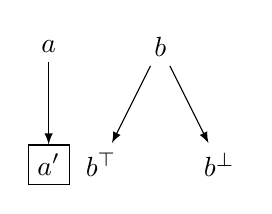
\begin{tikzpicture}[edge from parent/.style={draw,-latex}]
    %% \node[draw,circle,fill=violet!10] (circuit) {} child {
    %%   node[draw,circle,fill=violet!10] (bmaker) {$\diamondsuit$}
    %%   child {node[draw,circle,fill=violet!10] {}
    %%     child {node[draw,circle,fill=violet!10] {}}
    %%     child {node[draw,circle,fill=violet!10] {}
    %%       child {node[draw,circle,fill=violet!10] {}}
    %%       child {node[draw,circle,fill=violet!10] {}
    %%         child {node[draw,circle,fill=violet!10] {}}
    %%         child {node[draw,circle,fill=violet!10] (amaker) {$\heartsuit$}
    %%           child {node[draw,circle,fill=violet!10] (ref) {}
    %%             child {node[draw,circle,fill=violet!10] {}}
    %%           }
    %%         }
    %%       }
    %%     }
    %%   }
    %% };
    \node (a) {$a$} child {node[draw,rectangle] (aprime) {$a'$}};
    \node[right=1 cm of a] (b) {$b$}
    child {node (btop) {$b^\top$}}
    child {node (bbot) {$b^\bot$}};
    %% \node[draw,fit=(a) (aprime) (b) (btop) (bbot)] {};
    %% \draw[-latex] (ref) edge[densely dotted,bend left=90] (circuit);
    %% \draw[-latex,color=teal] (aprime) edge[densely dashed] node[xshift=2mm,color=teal] {$0$} (amaker);
    %% \draw[-latex,color=teal] (btop) edge[bend left=50,densely dashed] node[xshift=6mm,color=teal] {$0$} (bmaker);
    %% \draw[-latex,color=teal] (bbot) edge[bend left=50,densely dashed] node[yshift=-2mm,color=teal] {$1$} (bmaker);
  \end{tikzpicture}
  \caption{The forest of domains from \cref{example}. The directed edges correspond to the pairs of domains in $\pi$ but in the opposite direction, e.g., $\pi(a') = a$. The domain enclosed in a rectangle is the only domain created by constraint removal, i.e., $\mathcal{C} = \{\, a' \,\}$.}
  \label{fig:example}
\end{figure}

The function \texttt{traceAncestors} returns \texttt{null} if domain $d \in \mathcal{D}$ is not an ancestor of domain $e \in \mathcal{D}$. Otherwise, it returns \texttt{true} if the size of $e$ is guaranteed to be strictly smaller than the size of $d$ (i.e., there is domain created by the constraint removal rule on the path from $d$ to $e$) and \texttt{false} if their sizes will be equal at some point during inference.

Notation: For partial functions $\alpha, \beta\colon A \pfun B$ such that $\alpha|_{\dom(\alpha) \cap \dom(\beta)} = \beta|_{\dom(\alpha) \cap \dom(\beta)}$, we write $\alpha \cup \beta$ for the unique partial function such that $\alpha \cup \beta|_{\dom(\alpha)} = \alpha$, and $\alpha \cup \beta|_{\dom(\beta)} = \beta$.

\paragraph{TODO}
\begin{itemize}
\item introduce/describe \cref{alg:recursion} and \cref{alg:trycache} and describe the cache that's being used.
\item explain why $\rho \cup \gamma$ is possible
\item explain what the second return statement is about and why a third one is not necessary
\item mention which one is the main function, what each function takes and returns
\item explain the yield keyword
\item in the example below: write down both formula using the Forclift format
\item the parent relation and ancestor tracing is no longer necessary
\end{itemize}

The algorithm could be improved in two ways:
\begin{itemize}
\item by constructing a domain map first and then using it to reduce the number of viable variable bijections.
\item by similarly using the domain map $\rho$.
\end{itemize}
However, it is not clear that this would result in an overall performance improvement, since the number of variables in instances of interest never exceeds three and the identity bijection is typically the right one.

Diagramatically, \texttt{constructDomainMap} attempts to find $\gamma\colon \Doms(c) \to \Doms(d)$ such that the following diagram commutes (and returns \texttt{null} if such a function does not exist):
\[
\begin{tikzcd}
  \Vars(c) \ar[r, tail, two heads, "\beta"] \arrow[d, swap, "\delta_c"] & \Vars(d) \ar[d, "\delta_d"] \\
  \Doms(c) \ar[r, dashed, "\gamma"] \ar[d, hookrightarrow] & \Doms(d) \ar[d, hookrightarrow] \\
  \mathcal{D} \ar[r, swap, "\rho"] & \mathcal{D}.
\end{tikzcd}
\]

\begin{example} \label{example}
  Let $\phi$ be the formula
  \begin{align}
    \forall X \in a. \forall Y \in b. \forall Z \in b. Y \ne Z &\implies \neg p(X, Y) \lor \neg p(X, Z)\label{phi1} \\
    \forall X \in a. \forall Y \in b. \forall Z \in a. X \ne Z &\implies \neg p(X, Y) \lor \neg p(Z, Y).\label{phi2}
  \end{align}
  and $\psi$ be the formula
  \begin{align}
    \forall X \in a'. \forall Y \in b^\bot. \forall Z \in b^\bot. Z \ne Y &\implies \neg p(X, Y) \lor \neg p(X, Z)\label{psi1} \\
    \forall X \in a'. \forall Y \in b^\bot. \forall Z \in a'. X \ne Z &\implies \neg p(X, Y) \lor \neg p(Z, Y)\label{psi2}
  \end{align}

  The relevant domains and the definition of $\pi$ is in \cref{fig:example}. Since $\#\phi = \#\psi$, and the formulas are non-empty, the algorithm proceeds with the for-loops on \cref{line:for1,line:for2,line:generateMaps}. Suppose $c$ in the algorithm refers to \cref{phi1}, and $d$ to \cref{psi1}. Since both clauses have three variables, in the worst case, function \texttt{generateMaps} would have $3!=6$ bijections to check. Suppose the identity bijection is picked first. Then \texttt{constructDomainMap} is called with the following parameters:
  \begin{itemize}
  \item $V = \{\, X, Y, Z \,\}$,
  \item $\delta_c = \{\, X \mapsto a, Y \mapsto b, Z \mapsto b \,\}$,
  \item $\delta_d = \{\, X \mapsto a', Y \mapsto b^\bot, Z \mapsto b^\bot \,\}$,
  \item $\beta = \{\, X \mapsto X, Y \mapsto Y, Z \mapsto Z \,\}$,
  \item $\rho = \emptyset$.
  \end{itemize}
  Since $\delta_i(Y) = \delta_i(Z)$ for $i \in \{\, c, d \,\}$, \texttt{constructDomainMap} returns $\gamma = \{\, a \mapsto a', b \mapsto b^\bot \,\}$. Thus, \texttt{generateMaps} yields its first pair of maps $(\beta, \gamma)$ to \cref{line:generateMaps}. Furthermore, the pair satisfies $c[\beta, \gamma] = d$.

  Since $\pi(a') = a$, and $a' \in \mathcal{C}$, \texttt{traceAncestors($a$, $a'$)} returns \texttt{true}, which sets $\textsf{foundConstraintRemoval}'$ to \texttt{true} as well. When $e = b$, however, \texttt{traceAncestors}($b$, $b^\bot$) returns \texttt{false} since $b^\bot$ is a descendant of $b$ but not created by the constraint removal compilation rule. On \cref{line:recursion}, a recursive call to \texttt{identifyRecursion($\phi'$, $\psi'$, $\gamma$, true)} is made, where $\phi'$ and $\psi'$ are new formulas with one clause each: \cref{phi2} and \cref{psi2}, respectively.

  Again we have two non-empty formulas with equal hash codes, so \texttt{generateMaps} is called with $c$ set to \cref{phi2}, $d$ set to \cref{psi2}, and $\rho = \{\, a \mapsto a', b \mapsto b^\bot \,\}$. Suppose \cref{line:bijection} picks the identity bijection first again. Then \texttt{constructDomainMap} is called with the following parameters:
  \begin{itemize}
  \item $V = \{\, X, Y, Z \,\}$,
  \item $\delta_c = \{\, X \mapsto a, Y \mapsto b, Z \mapsto a \,\}$,
  \item $\delta_d = \{\, X \mapsto a', Y \mapsto b^\bot, Z \mapsto a' \,\}$,
  \item $\beta = \{\, X \mapsto X, Y \mapsto Y, Z \mapsto Z \,\}$,
  \item $\rho = \{\, a \mapsto a', b \mapsto b^\bot \,\}$.
  \end{itemize}
  Since $\beta$ and $\rho$ `commute' (TODO: as in the diagram above), and there are no new domains in $\Doms(c)$ and $\Doms(d)$, $\gamma$ exists and is equal to $\rho$. Again, the returned pair $(\beta, \gamma)$ satisfies $c[\beta, \gamma] = d$. This $\gamma$ passes the \texttt{traceAncestors} checks exactly the same way as the one before, and \cref{line:recursion} calls \texttt{identifyRecursion($\emptyset$, $\emptyset$, $\rho$, true)}, which immediately returns $\rho = \{\, a \mapsto a', b \mapsto b^\bot \,\}$ as the final answer. This means that one can indeed use a circuit for $\WMC(\phi)$ to compute $\WMC(\psi)$ by replacing every mention of $a$ with $a'$ and every mention of $b$ with $b^\bot$.
\end{example}

\subsection{Evaluation}

$\WMC(\Reff_\rho(n); \size) = \WMC(n; \size')$ ($n$ is the target circuit node), where $\size'$ is defined as
\[
\size'(x) =
\begin{cases}
  \size(\rho(x)) & \text{if } x \in \dom(\rho) \\
  \size(x) & \text{otherwise}
\end{cases}
\]
for all $x \in \mathcal{D}$.

\section{New Operations}

\subsection{Constraint Removal}

TODO: introduce the Forclift-style notation (e.g., the compile operator) and the arbitrary formula $\phi$.

\paragraph{Preconditions.} There is a domain $d \in \mathcal{D}$ and an element $e \in d$ such that:
\begin{itemize}
\item for each clause $c = (L, C, \delta_c) \in \phi$ and variable $v \in \Vars(c)$, either $\delta_c(v) \ne d$ or $(v, e) \in C$;
\item $e$ does not occur in any literal of any clause of $\phi$.
\end{itemize}

\paragraph{Operator.} First, we introduce a new domain (i.e., $\mathcal{D} \coloneqq \mathcal{D} \sqcup \{\, d' \,\}$), add it to $\mathcal{C}$ (i.e., $\mathcal{C} \coloneqq C \sqcup \{\, d' \,\}$), and set $\pi(d') \coloneqq d$. Then $\CR(\phi) = \CR_{d \mapsto d'}(\Compile(\phi'))$. The new formula $\phi'$ is defined by replacing every clause $(L, C, \delta) \in \phi$ by a clause $c' = (L, C', \delta') \in \phi'$, where
\[
C' = \{\, (x, y) \in C \mid y \ne e \,\},
\]
and
\[
\delta'(x) =
\begin{cases}
  d' & \text{if } \delta(x) = d \\
  \delta(x) & \text{otherwise}
\end{cases}
\]
for all $x \in \Vars(c') \subseteq \Vars(c)$.

\begin{example}
  Let $\phi = \{\, c_1, c_2, c_e \,\}$ be a formula with clauses (constants lowercase, variables uppercase)
  \begin{align*}
    c_1 &= (\emptyset, \{\, (Y, X) \,\}, \{\, X \mapsto b^\top, Y \mapsto b^\top \,\}), \\
    c_2 &= (\{\, \neg p(X, Y), \neg p(X, Z) \,\}, \{\, (X, x), (Y, Z) \,\}, \{\, X \mapsto a, Y \mapsto b^\bot, Z \mapsto b^\bot \,\}), \\
    c_3 &= (\{\, \neg p(X, Y), \neg p(Z, Y) \,\}, \{\, (X, x), (Z, X), (Z, x) \,\}, \{\, X \mapsto a, Y \mapsto b^\bot, Z \mapsto a \,\}).
  \end{align*}
  Domain $a$ and with its element $x \in a$ satisfy the preconditions for constraint removal. The operator introduces a new domain $a'$ and transforms $\phi$ to $\phi' = (c_1', c_2', c_3')$, where
  \begin{align*}
    c_1' &= c_1 \\
    c_2' &= (\{\, \neg p(X, Y), \neg p(X, Z) \,\}, \{\, (Y, Z) \,\}, \{\, X \mapsto a', Y \mapsto b^\bot, Z \mapsto b^\bot \,\}) \\
    c_3' &= (\{\, \neg p(X, Y), \neg p(Z, Y) \,\}, \{\, (Z, X) \,\}, \{\, X \mapsto a', Y \mapsto b^\bot, Z \mapsto a' \,\}).
  \end{align*}
\end{example}

\paragraph{Evaluation.}
\[
\WMC(\CR_{d \mapsto d'}(n); \size) =
\begin{cases}
  \WMC(n; \size \cup \{\, d' \mapsto \size(d) - 1 \,\}) & \text{if } \size(d) > 0 \\
  0 & \text{otherwise.}
\end{cases}
\]

\subsection{A Generalisation of Domain Recursion}

\begin{algorithm}[t]
  \caption{Formula transformation for domain recursion}
  \label{alg:domainrecursion}
  \KwIn{formula $\phi$, domain $d \in \mathcal{D}$, and constant $x$}
  \KwOut{formula $\phi'$}
  $\phi' \gets \emptyset$\;
  \ForEach{clause $c = (L, C, \delta) \in \phi$\label{line:forclause}}{
    $V \gets \{\, v \in \Vars(L) \mid \delta(v) = d \,\}$\;
    \ForEach{subset $W \subseteq V$ such that $W^2 \cap C = \emptyset$ {\bf and} $W \cap \{\, v \in \Vars(C) \mid (v, y) \in C \text{ for some constant } y \,\} = \emptyset$\label{line:conditions}}{
      \tcc{Here, $\delta'$ is the restriction of $\delta$ to the new set of variables}
      $\phi' \gets \phi' \cup \{\, (L[x/W], C[x/W] \cup \{\, (v, x) \mid (v \in V \setminus W) \,\}, \delta') \,\}$\;
    }
  }
\end{algorithm}

TODO: Compare with the original. The original version of domain recursion is here \cite{DBLP:conf/nips/Broeck11}.

TODO: introduce $\phi$.

\paragraph{Precondition.} Domain recursion can be applied to domain $d \in \mathcal{D}$ if there is a clause $c$ with a literal variable $v \in \Vars(L_c)$ such that $\delta_c(v) = d$.

\paragraph{Operator.} First, introduce a new constant $x$. Then $\DR(\phi) = \DR_d(\Compile(\phi'))$, where $\phi'$ is generated by \cref{alg:domainrecursion}.

\begin{example}
  Let $\phi = \{\, c_1, c_2 \,\}$ be a formula, where
  \begin{align*}
    c_1 &= (\{\, \neg p(X, Y), \neg p(X, Z) \,\}, \{\, (Z, Y) \,\}, \{ X \mapsto a, Y \mapsto b, Z \mapsto b \}), \\
    c_2 &= (\{\, \neg p(X, Y), \neg p(Z, Y) \,\}, \{\, (Z, X) \,\}, \{ X \mapsto a, Y \mapsto b, Z \mapsto a \}).
  \end{align*}
  While domain recursion is possible on both domains, here we illustrate how it works on $a$.

  Suppose \cref{line:forclause} picks $c = c_1$ first. Then $V = \{\, X \,\}$. Both subsets of $V$ satisfy the conditions on \cref{line:conditions} and generate new clauses
  \[
  (\{\, \neg p(X, Y), \neg p(X, Z) \,\}, \{\, (Z, Y), (X, x) \,\}, \{ X \mapsto a, Y \mapsto b, Z \mapsto b \}),
  \]
  (from $W = \emptyset$) and
  \[
  (\{\, \neg p(x, Y), \neg p(x, Z) \,\}, \{\, (Z, Y) \,\}, \{ Y \mapsto b, Z \mapsto b \})
  \]
  (from $W = V$).

  When $c = c_2$, then $V = \{\, X, Z \,\}$. The subset $W = V$ fails to satisfy the first condition because of the $Z \ne X$ constraint; without this condition, the resulting clause would have an unsatisfiable constraint $x \ne x$. The other three subsets of $V$ all generate clauses for $\phi'$:
  \[
  (\{\, \neg p(X, Y), \neg p(Z, Y) \,\}, \{\, (Z, X), (X, x), (Z, x) \,\}, \{ X \mapsto a, Y \mapsto b, Z \mapsto a \})
  \]
  (from $W = \emptyset$),
  \[
  (\{\, \neg p(x, Y), \neg p(Z, Y) \,\}, \{\, (Z, x) \,\}, \{ Y \mapsto b, Z \mapsto a \})
  \]
  (from $W = \{\, X \,\}$), and
  \[
  (\{\, \neg p(X, Y), \neg p(x, Y) \,\}, \{\, (X, x) \,\}, \{ X \mapsto a, Y \mapsto b, \})
  \]
  (from $W = \{\, Z \,\}$).
\end{example}

\paragraph{Evaluation.}
\[
\WMC(\DR_d(n); \size) =
\begin{cases}
  \WMC(n; \size) & \text{if } \size(d) > 0 \\
  1 & \text{otherwise.}
\end{cases}
\]

One is picked as the multiplicative identity.

\section{Other Topics}

\begin{itemize}
\item new rules that don't create nodes (e.g., duplicate removal, unconditional contradiction detection, etc.)
\item some notes on halting
  \begin{itemize}
  \item Search is infinite. Some rules increase the size of the formula(s), but most reduce it.
  \item Inference is guaranteed to terminate if at least one domain shrinks by at least one. But note that allowing recursive calls with the same domain sizes (e.g., $f(n) = f(n) + \dots$) could be useful because these problematic terms might cancel out.
  \item It's impossible for $n \gets n - 1$ and $\texttt{for } n \in \dots$ to combine in a way that results in an infinite loop.
  \end{itemize}
\end{itemize}

\section{Circuit Nodes Types and Their Evaluations}

Along with the three circuit node types described above, here are all the other ones. This section is mostly just taken from \cite{DBLP:conf/ijcai/BroeckTMDR11} but with some changes in notation.

TODO: explain that $x, y, z$ refer to nodes, $c$ refers to a clause, and describe each node type in a bit more detail.

\begin{description}
\item[tautology] $\WMC(\Tautology; \size) = 1$
\item[contradiction] $\WMC(\Contradiction c; \size) = 0^{\gr(c; \size)}$
\item[unit clause]
  \[
  \WMC(\Unit c; \size) =
  \begin{cases}
    \wwp(p)^{\gr(c; \size)} & \text{if the literal is positive} \\
    \wwn(p)^{\gr(c; \size)} & \text{otherwise,}
  \end{cases}
  \]
  where $p$ is the predicate of the literal.
\item[smoothing] $\WMC(\Smoothing c; \size) = (\wwp(p) + \wwn(p))^{\gr(c; \size)}$, where $p$ is the predicate of the literal.
\item[decomposable conjunction] $\WMC(x \oland y; \size) = \WMC(x; \size) \times \WMC(y; \size)$
\item[deterministic disjunction] $\WMC(x \olor y; \size) = \WMC(x; \size) + \WMC(y; \size)$
\item[decomposable set-conjunction] $\WMC(\oland_D x; \size) = \WMC(x; \size)^{\size(D)}$
\item[deterministic set-disjunction] $\WMC(\olor_{D \subseteq S} x; \size) = \sum_{d = 0}^{\size(S)} \binom{\size(S)}{d} \WMC(x; \size \cup \{\, D \mapsto d \,\})$
\item[inclusion-exclusion] $\WMC(\IE(x, y, z); \size) = \WMC(x; \size) + \WMC(y; \size) - \WMC(z; \size)$
\end{description}

\subsection{Observations and Theoretical Results}

TODO: explain how circuits and domain sizes connect to functions on integers

\begin{observation}
  Let $n$ be a positive integer and $d \in \mathcal{D}$ a domain. Then one can construct a circuit $x$ such that
  \[
  \WMC(x; \size) =
  \begin{cases}
    0 & \text{if } \size(d) \ge n \\
    \WMC(y; \size) & \text{otherwise,}
  \end{cases}
  \]
  where $y$ is a circuit node of arbitrary type. Indeed, $(\Contradiction c) \oland y$ is such a circuit, where $c = (L, C, \delta)$ is a clause with $n$ variables $(v_i)_{i=1}^n$ such that:
  \begin{itemize}
  \item $L$ is unimportant,
  \item $C = \{\, (v_i, v_j) \mid i = 1, \dots, n - 1\text{, }j = i + 1, \dots, n \,\}$,
  \item and $\delta(v_i) = d$ for all $i = 1, \dots, n$.
  \end{itemize}
  TODO: explain why this works.
\end{observation}

\begin{remark}
  Such (sub)circuits can be constructed automatically using compilation rules, although $n$ is upper bounded by the maximum number of variables in any clause of the input formula since there is no rule that would introduce new variables.
\end{remark}

\section{Examples}

For both one domain and two domains:
\begin{itemize}
\item bijections
\item injections
\item partial injections
\end{itemize}

\section{Conclusions and Future Work}

\begin{itemize}
\item Transform circuits to definitions of (possibly recursive) functions on integers. Use a computer algebra system to simplify them.
\item Design an algorithm to infer the necessary base cases. (Note that there can be an infinite amount of them when functions have more than one parameter.)
\end{itemize}

\bibliographystyle{acm}
\bibliography{notes}

\end{document}
